%%%%%%%%%%%%%%%%%%%%%%%%%%%%%%%%%%%%%%%%%%%%%%%%%%%%%%%%%%%%%%%%%%%%%%%%%%%%%%%%
%2345678901234567890123456789012345678901234567890123456789012345678901234567890
%        1         2         3         4         5         6         7         8

\documentclass[letterpaper, 10 pt, conference]{ieeeconf}  % Comment this line out if you need a4paper

\usepackage{hyperref}
\usepackage{graphicx}
%\usepackage{subfig}
\usepackage{caption}
\usepackage{subcaption}
\usepackage{mathtools}
\usepackage{algorithm2e}
%\documentclass[a4paper, 10pt, conference]{ieeeconf}      % Use this line for a4 paper

\IEEEoverridecommandlockouts                              % This command is only needed if 
                                                          % you want to use the \thanks command

\overrideIEEEmargins                                      % Needed to meet printer requirements.

% See the \addtolength command later in the file to balance the column lengths
% on the last page of the document

% The following packages can be found on http:\\www.ctan.org
%\usepackage{graphics} % for pdf, bitmapped graphics files
%\usepackage{epsfig} % for postscript graphics files
%\usepackage{mathptmx} % assumes new font selection scheme installed
%\usepackage{times} % assumes new font selection scheme installed
%\usepackage{amsmath} % assumes amsmath package installed
%\usepackage{amssymb}  % assumes amsmath package installed



\title{\LARGE \bf
Efficient Collision Avoidance and Trajectory Adjustment for DRC-Hubo
}


\author{Michael Grey% <-this % stops a space
%\thanks{$^{1}$Albert Author is with Faculty of Electrical Engineering, Mathematics and Computer Science,
%        University of Twente, 7500 AE Enschede, The Netherlands
%        {\tt\small albert.author@papercept.net}}%
%\thanks{$^{2}$Bernard D. Researcheris with the Department of Electrical Engineering, Wright State University,
%        Dayton, OH 45435, USA
%        {\tt\small b.d.researcher@ieee.org}}%
}


\begin{document}



\maketitle
\thispagestyle{empty}
\pagestyle{empty}


%%%%%%%%%%%%%%%%%%%%%%%%%%%%%%%%%%%%%%%%%%%%%%%%%%%%%%%%%%%%%%%%%%%%%%%%%%%%%%%%
\begin{abstract}

The author uses a Jacobian-based collision avoidance algorithm which leverages convex collision geometries to detect and escape collisions prior to them happening. The algorithm is efficient enough to be run in real time, but can also be used to adjust an existing trajectory prior to execution. The focus of this algorithm is on efficiency and makes no attempt to offer any guarantees on completeness or optimality. 

\end{abstract}


%%%%%%%%%%%%%%%%%%%%%%%%%%%%%%%%%%%%%%%%%%%%%%%%%%%%%%%%%%%%%%%%%%%%%%%%%%%%%%%%
\section{INTRODUCTION}

Collision avoidance is of critical importance for high degree-of-freedom robots, because physical collisions can result in damage to the robot, the environment, or even human beings in the workspace of the robot. Motion planning algorithms can be used to generate collision-free paths for robot links. These algorithms can be complete \cite{Lozano} or probabilistically complete \cite{PRM}\cite{RRT}. Alternatively, collision avoidance can be handled on a lower level, for example using the concept of artificial potential fields \cite{Khatib}.

Complete and probabilistically complete motion plan generation for high-dimensional configuration spaces is computationally expensive, sometimes to the point of not being viable. Moreover, the human safety aspect demands that the ability to detect and avoid collisions rapidly. A planner which requires a run-time that exceeds real-time speeds is not an acceptable method for handling these critical situations. If a trajectory needs to be replanned in order to handle an unexpected collision (for example, a newly introduced obstacle in the environment), it would be undesirable to use a sampling-based motion planner that might take arbitrarily long to produce a solution. 

Instead, for the sake of efficiency, this paper explores an algorithm analogous to the artificial potential field concept of Khatib \cite{Khatib} except that it does not use the potential fields to achieve a particular goal configuration. In this paper, potential fields are merely used to adjust an existing trajectory, and they only exist when the collision geometry of the robot intersects itself or an obstacle. The premise is that a planner (or some other source) has generated a trajectory to be executed on the robot, but a new obstacle was introduced some time after the plan was generated (for example, at runtime). After the potential field adjustment, cubic splines are used to cleanly and efficiently mesh a collision-free trajectory segment into the original trajectory. This can be useful if an arbitrary trajectory is provided without any knowledge of the trajectory's objective function or goal, but the trajectory needs to be resolved to avoid collisions with minimal changes to its overall path and end configuration.



\section{METHODS}

There are three primary components to the algorithm used for this project. At the end of this section we provide an overview for how these components work together.

\subsection{Convex Continuous Collision Detection}

The first key component of the algorithm is the ability to continuously detect collisions between convex geometries. This was noted as a requirement by Khatib for the use of potential fields \cite{Khatib}. To this end, the algorithm uses libccd\footnote{Information on libccd can be found here: \url{http://libccd.danfis.cz/about}}. ``Continuous collision detection'' in this context means that, in addition to simply identifying when a collision occurs, we know which point on each geometry most deeply intersects the offending geometry. This also means that we have a vector to indicate what direction each geometry could be moved in to reduce the amount of collision, as seen in Fig. \ref{fig:thigh_punch_collision}. 

\begin{figure}[h]
    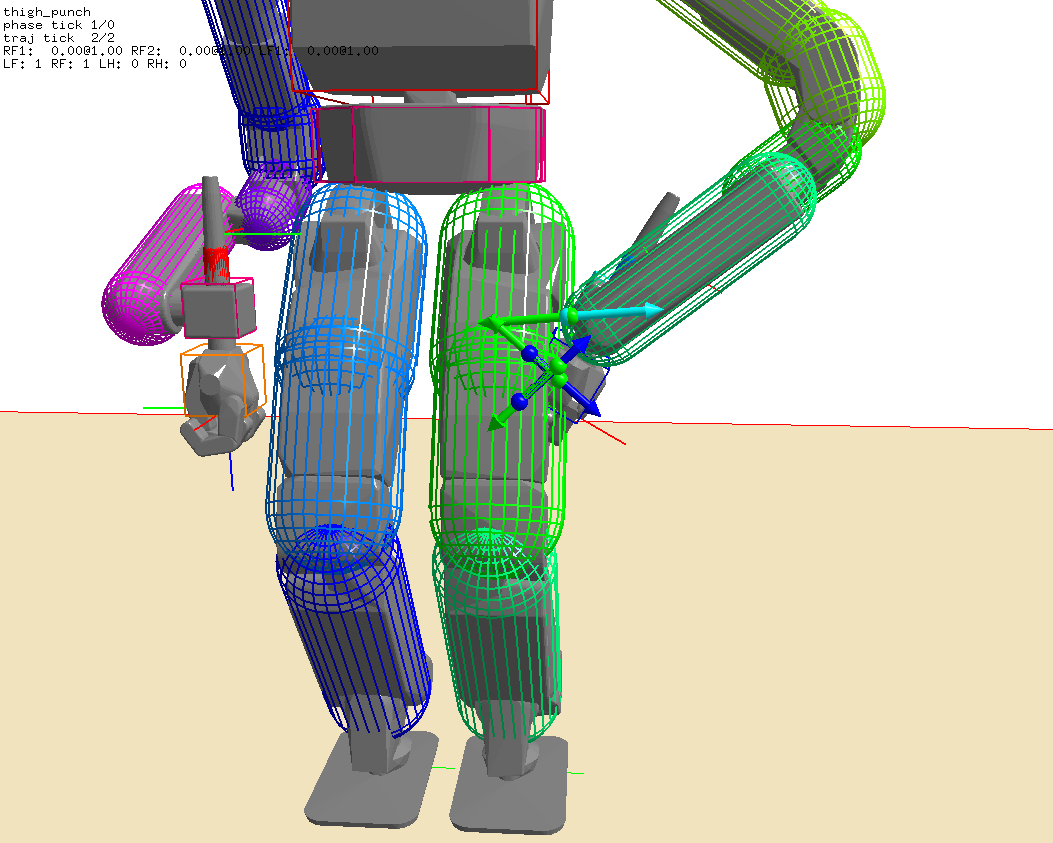
\includegraphics[width=\columnwidth]{pictures/thigh_punch_collision}
    \caption{Collision geometry and collision normals of the left fist in the left thigh}
    \label{fig:thigh_punch_collision}
\end{figure}

The collision geometries are generally represented as spheres, capsules (a.k.a. pills or cylinders with spherical caps), and boxes. These are simple convex shapes which do a respectable job of encapsulating the complex geometry of the robot. By combining these shapes in clever ways, they can offer a good compromise between accuracy, safety buffer, and efficiency. In Fig. \ref{fig:col_geoms} we see the collision geometries of various body parts (represented by the technicolor lines and curves, \emph{not} the solid model). The arm is long and slender, so it uses mostly capsules to represent its volume (Fig. \ref{fig:arm_col_geoms}. The actual chest is close to being a cube, so that is encapsulated with one large box (Fig. \ref{fig:chest_col_geom}). In order to get the many-sided polygon for the pelvis (Fig. \ref{fig:pelvis_col_geom}) a series of boxes are strung together at angles with each other. It may seem like a strange approach for constructing complicated shapes, but it allows the collision detection library to make assumptions that provide quick analytical results for continuous collision detection. It is usually okay--sometimes even desirable--to sloppily overestimate the physical volume of the robot links, as long as the overestimation does not produce false negatives that impede viable solutions. 

\begin{figure}[h]
    \centering
    \begin{subfigure}[h]{1.0\columnwidth}
        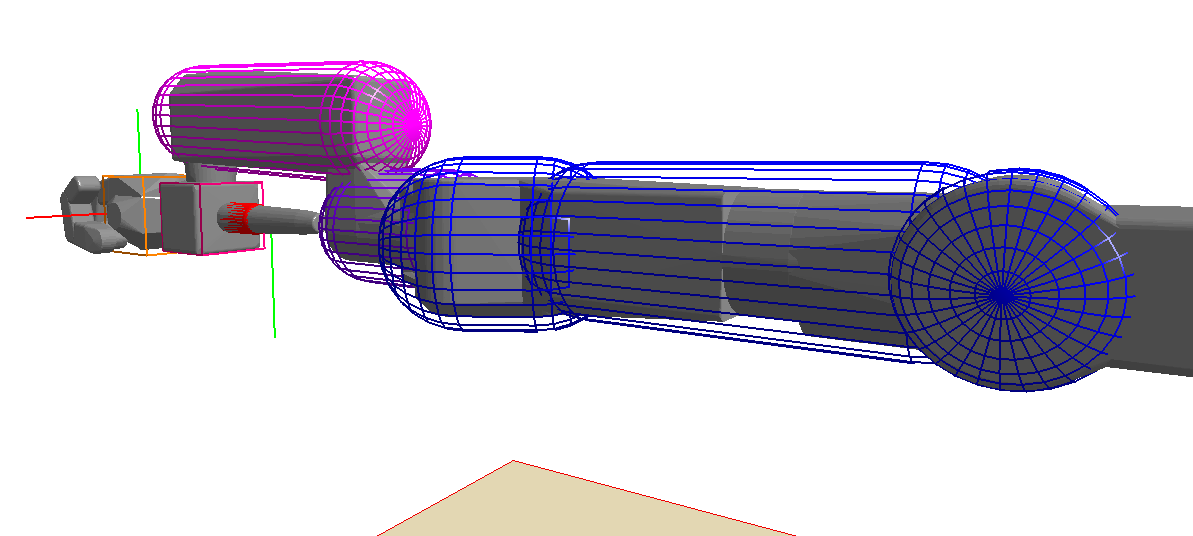
\includegraphics[width=\columnwidth]{pictures/arm_col_geom}
        \caption{Arm collision geometries}
        \label{fig:arm_col_geoms}
    \end{subfigure}
    \begin{subfigure}[h]{0.45\columnwidth}
        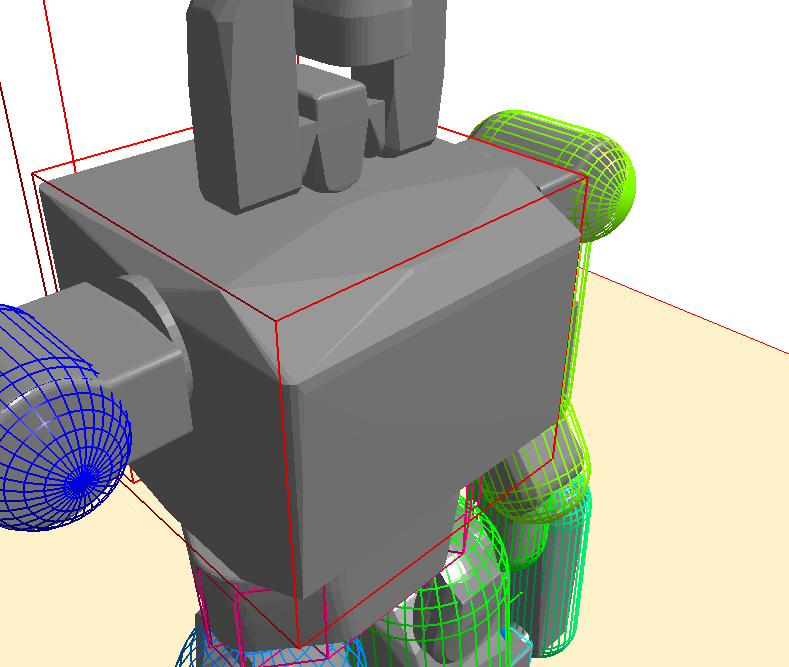
\includegraphics[width=\columnwidth]{pictures/chest_col_geom}
        \caption{Chest collision geometries}
        \label{fig:chest_col_geom}
    \end{subfigure}
    \begin{subfigure}[h]{0.45\columnwidth}
        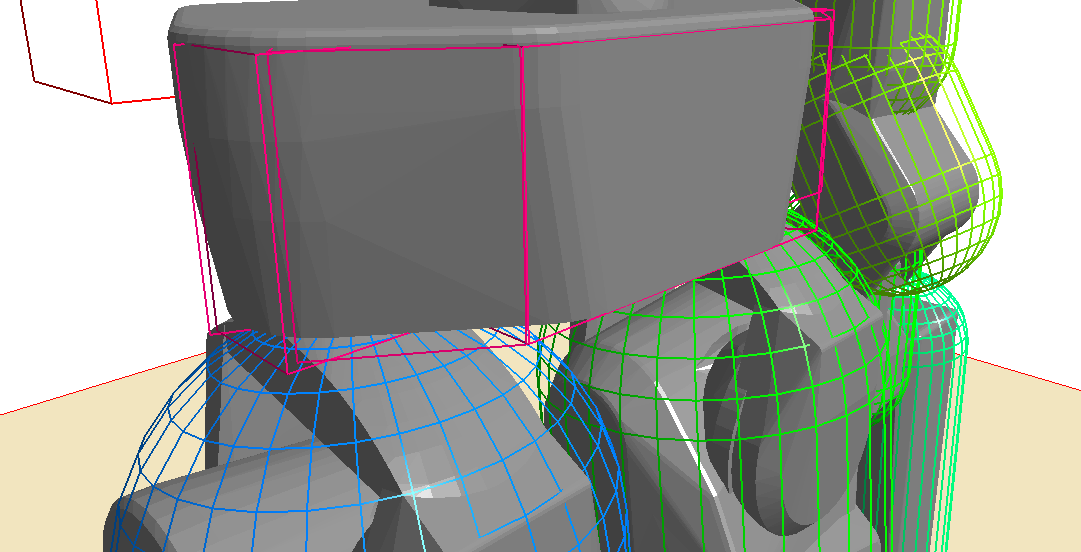
\includegraphics[width=\columnwidth]{pictures/pelvis_col_geom}
        \caption{Pelvis collision geometries}
        \label{fig:pelvis_col_geom}
    \end{subfigure}
    \caption{Collision geometries of various parts of the robot}
    \label{fig:col_geoms}
\end{figure}

\subsection{Jacobian Descent}

Leveraging the continuous collision detection, we can use the pseudo-inverse Jacobian to find a joint configuration which is close to the original but collision-free. The Jacobian of a robot kinematic chain describes the mapping from joint speeds to end effector speeds. In this case, the "end-effector" can be thought of as any kinematic body which is in collision. So if the elbow is in collision, we treat the elbow frame as the end-effector frame (even though traditionally the hand of the robot would be considered its end-effector). We take the Jacobian which leads from the root of the kinematic tree up to the object which is in collision and use that to inform our iterative procedure.

Specifically, a damped least squares pseudo-inverse Jacobian\footnote{An excellent explanation of inverse kinematics can be found at this website: \url{http://www.math.ucsd.edu/~sbuss/ResearchWeb/ikmethods/iksurvey.pdf}} is used to calculate changes in joint angles. This takes the form of Eq. \ref{eq:PIJ} where $J_{c}$ is the Jacobian of the point which is in collision, $\Delta \vec{\theta}$ is the change in joint angles, $\Delta \vec{x}$ is the desired displacement, and $\lambda$ is an arbitrary damping factor (0.05 was chosen for this project). Note that Jacobians are often used to control both end effector translation and orientation, but in this case we only care about translating the links away from collisions and are unconcerned about their rotation. Therefore, we ignore the rotational components of the Jacobian.

\begin{equation}
    \Delta \vec{\theta} = J_{c}^{T} ( J_{c} J_{c}^{T} + \lambda^{2} I )^{-1} \Delta \vec{x} 
%    \caption{Damped least squares pseudo-inverse Jacobian method}
    \label{eq:PIJ}
\end{equation}

The Jacobian is used to progressively iterate the geometries out of their collisions. Each step taken through the Jacboian is clamped down to a 5$mm$ step. This step size is arbitrary, but it reflects a practical compromise between precision and efficiency. The attempt to resolve a particular collision terminates after 1000 iterations (again, an arbitrary value, but reflects a good balance), and the solver moves on to the next collision in the list hoping that solving for a different collision will resolve the first one. An alternative approach might attempt to address every collision in each iteration, but this runs a great risk of getting ``cornered'' in a local minimum where two collisions have opposing normals.

Additionally, we may be interested in preserving the pose of the manipulator (a.k.a. the robot's hand) while still moving the links of the arm out of collisions (assuming the manipulator itself is not presently in a collision). For this purpose, we can project $\Delta \vec{\theta}$ through the nullspace of manipulator's Jacobian. In order to find the nullspace of the manipulators' Jacobians, we employ the JacobiSVD found in the Eigen C++ library\footnote{More information on Eigen C++ can be found here: \url{http://eigen.tuxfamily.org/index.php?title=Main_Page}}. The JacobiSVD class produces a V Matrix which has columns that correspond to zero-valued singular values. These zeroed singular values form the basis of the Jacobian's nullspace, because they indicate vectors of joint angle changes which do not effect the pose of the manipulator. By simply extracting the block of the V Matrix corresponding to zero singular values and projecting the afrorementioned $\Delta \vec{\theta}$ through this basis, we get values of $\Delta \vec{\theta_{ns}}$ which move the links in the kinematic chain without moving the manipulator.

\subsection{Cubic Splines}

The final key component of the method used is cubic splining. Cubic splines have useful properties for efficiently interpolating full body trajectories. Specifically, it is possible to dictate the initial and final position and velocity of a cubic spline. And even more crucially, there are analytical solutions for how to scale a cubic spline in order to achieve a given maximum velocity or acceleration. Velocity and acceleration limits are of critical importance for robot applications since exceeding these limits can result in damage to the robot or the robot's environment. Cubic splines offer a single framework which allows us to efficiently make continuously differentiable corrections to trajectories.

When altering a full body trajectory for a humanoid robot like the DRC-Hubo, it is critical to ensure that the entire body moves synchronously. If, for example, an arm needs to be slowed down in order to avoid a collision, it is important that the entire body be slowed down in sync with it, for two particular reasons

\begin{itemize}
\item The body needs to maintain balance. Full body trajectories for humanoid robots are (ideally) generated in such a way that they remain balanced. If a subset of the joints in the trajectory are sped up or slowed down, it might destroy assumptions made by the original trajectory in order to maintain balance.
\item A trajectory might have been designed with kinematic constraints between different manipulators (or between the feet supporting it), and these kinematic constraints are likely to be violated if one manipulator moves faster than the other. For example, if both hands are holding the same object, their velocities need to match each other, or the robot will not be able to maintain a hold on the object (and will potentially break the object or break itself).
\end{itemize}

When altering a trajectory, we consider the strictest velocity/acceleration limit on the robot--in other words, the velocity (or acceleration) limit which results in the most time required to transition from the start configuration to the end configuration. This limit is used to inform the necessary interpolation time for the cubic spline. Equations \ref{eq:max_vel} and \ref{eq:max_accel} indicate the relationship between velocity / acceleration limits and the time necessary for interpolation. $T_{max\_vel}$ is the length of time required to satisfy the maximum velocity limit of a feature, $T_{max\_accel}$ is the lenght of time required to satisfy the acceleration limit of a feature, $D$ is the total displacement of the feature from the start to the end, $V_{max}$ is the feature's maximum velocity, and $A_{max}$ is the feature's maximum acceleration. $v_0$ is the initial (and final) \emph{unitless} velocity. Unitless means that it is scaled to the velocity of some other cubic spline, and it can range from 0 to 1.5 (because 1.5 is the maximum velocity of a cubic spline which goes from 0 to 1 while beginning and ending with 0 velocity).

\begin{equation}
    T_{max\_vel} = \frac{(3 - v_{0})D}{2 V_{max}}
    \label{eq:max_vel}
\end{equation}

\begin{equation}
    T_{max\_accel} = \sqrt{ \left| \frac{6(1-v_{0})D}{A_{max}} \right| }
    \label{eq:max_accel}
\end{equation}

For our purposes, the cubic splines will always have the same initial and final velocity, although this is not an inherent requirement of cubic splines. We do this because a complete trajectory must always begin and end with zero velocity (i.e. the same velocity), and when we modify a trajectory, it is desirable for our modified segment to end with the same velocity that it began with in order to be continuous and allow the rest of the trajectory to behave as it originally expected. In this way, we can ensure that we continue to respect velocity and acceleration limits while still avoiding collisions. Fig. \ref{fig:splines} displays the complete range of splines which are permitted by the algorithm.

\begin{figure}[h]
    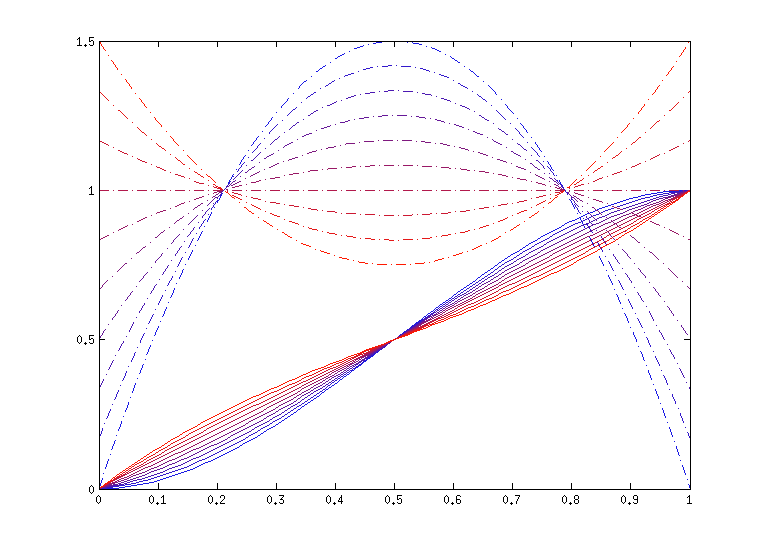
\includegraphics[width=\columnwidth]{pictures/splines}
    \caption{Splines with varying initial (unitless) velocities: blue=0, red=1.5. Dashed lines represent the corresponding first-order derivatives.}
    \label{fig:splines}
\end{figure}

\subsection{Complete Algorithm}

The algorithm which combines the above three components can be expressed with the following pseudo-code.

\begin{algorithm}

    \SetLine
    \KwData{$collision\_list$, $robot\_state$}
    \While{collision\_list.notEmpty()} {
        \For{ collision $\leftarrow$ collision\_list } {
            $J_{c}$ $\leftarrow$ Jacobian($collision$, $robot\_state$)\;
            $J_{c}^{-1}$ $\leftarrow$ dampedPseudoInverse($J_{c}$)\;
            $\Delta \vec{\theta}$ $\leftarrow$ $J_{c}^{-1}$ * $collision$.normal\_vector()\;
            \For{ manip $\leftarrow$ manipulator\_list } {
                \If{collision != manip} {
                    $J_{m}$ $\leftarrow$ Jacobian($manip$, $robot\_state$)\;
                    $\Delta \vec{\theta}$ $\leftarrow$ nullspaceProjection($J_{m}$, $\Delta \vec{\theta}$)\;
                }
            }
            $robot\_state$ $\leftarrow$ apply($\Delta \vec{\theta}$, $robot\_state$)\;
            $attempt$++\;
            \If{$attempt$ $\geq$ $maxAttempts$} {
                return $false$\;
            }
        }
    }
    return $true$\;

\end{algorithm}

\subsection{Experiments}

There are three scenarios which are of primary concern for this algorithm

\begin{itemize}
\item The end effector has been instructed to run through an obstacle.



\section{USING THE TEMPLATE}

Use this sample document as your LaTeX source file to create your document. Save this file as {\bf root.tex}. You have to make sure to use the cls file that came with this distribution. If you use a different style file, you cannot expect to get required margins. Note also that when you are creating your out PDF file, the source file is only part of the equation. {\it Your \TeX\ $\rightarrow$ PDF filter determines the output file size. Even if you make all the specifications to output a letter file in the source - if your filter is set to produce A4, you will only get A4 output. }

It is impossible to account for all possible situation, one would encounter using \TeX. If you are using multiple \TeX\ files you must make sure that the ``MAIN`` source file is called root.tex - this is particularly important if your conference is using PaperPlaza's built in \TeX\ to PDF conversion tool.

\subsection{Headings, etc}

Text heads organize the topics on a relational, hierarchical basis. For example, the paper title is the primary text head because all subsequent material relates and elaborates on this one topic. If there are two or more sub-topics, the next level head (uppercase Roman numerals) should be used and, conversely, if there are not at least two sub-topics, then no subheads should be introduced. Styles nprescribed.

\subsection{Figures and Tables}

Positioning Figures and Tables: Place figures and tables at the top and bottom of columns. Avoid placing them in the middle of columns. Large figures and tables may span across both columns. Figure captions should be below the figures; table heads should appear above the tables. Insert figures and tables after they are cited in the text. Use the ab even at the beginning of a sentence.

\begin{table}[h]
\caption{An Example of a Table}
\label{table_example}
\begin{center}
\begin{tabular}{|c||c|}
\hline
One & Two\\
\hline
Three & Four\\
\hline
\end{tabular}
\end{center}
\end{table}


   \begin{figure}[thpb]
      \centering
      \framebox{\parbox{3in}{We suggest that you use a text box to insert a graphic (which is ideally a 300 dpi TIFF or EPS file, with all fonts embedded) because, in an document, this method is somewhat more stable than directly inserting a picture.
}}
      %\includegraphics[scale=1.0]{figurefile}
      \caption{Inductance of oscillation winding on amorphous
       magnetic core versus DC bias magnetic field}
      \label{figurelabel}
   \end{figure}
   

Figure Labels: Use 8 point Times New Roman for Figure labels. Use words rather than symbols or abbreviations when writing Figure axis labels to avoid confusing the reader. As an example, write the qutincluding units inatio

\section{CONCLUSIONS}

A conclusion section is not required. Although a conclusion may review the main points of the paper, do not replicate the abstract as the conclusion. A conclusion might elaborate on the importance of the work or suggest applications and extensions. 

\addtolength{\textheight}{-12cm}   % This command serves to balance the column lengths
                                  % on the last page of the document manually. It shortens
                                  % the textheight of the last page by a suitable amount.
                                  % This command does not take effect until the next page
                                  % so it should come on the page before the last. Make
                                  % sure that you do not shorten the textheight too much.

%%%%%%%%%%%%%%%%%%%%%%%%%%%%%%%%%%%%%%%%%%%%%%%%%%%%%%%%%%%%%%%%%%%%%%%%%%%%%%%%



%%%%%%%%%%%%%%%%%%%%%%%%%%%%%%%%%%%%%%%%%%%%%%%%%%%%%%%%%%%%%%%%%%%%%%%%%%%%%%%%



%%%%%%%%%%%%%%%%%%%%%%%%%%%%%%%%%%%%%%%%%%%%%%%%%%%%%%%%%%%%%%%%%%%%%%%%%%%%%%%%
\section*{APPENDIX}

Appendixes should appear before the acknowledgment.

\section*{ACKNOWLEDGMENT}

Many thanks to Matt Zucker who provided the collision detection, kinematics, and visualization environment that made this project possible.


%%%%%%%%%%%%%%%%%%%%%%%%%%%%%%%%%%%%%%%%%%%%%%%%%%%%%%%%%%%%%%%%%%%%%%%%%%%%%%%%

References are important to the reader; therefore, each citation must be complete and correct. If at all possible, references should be commonly available publications.



%\begin{thebibliography}{99}
%\end{thebibliography}

\bibliographystyle{IEEEtran}
\bibliography{bibliography}



\end{document}
